\chapter{Cost functions, binary classifiers, and performance measures}
\section{Cost functions}
\lecture{4}{3/2}

\begin{definition}[Cost function]
    A \textbf{loss function} (or \textbf{cost function})
    is a function that maps values of variables onto $\R$
    intuitively representing the \emph{cost} of the set.
\end{definition}

In our case, a cost function will describe how well the current
\emph{response surface} $h(x)$ fits the available data, defined as:
\[
    J(y_i, h(x_i))
\]
where $y_i$ is the observed value and $h(x_i)$ is the predicted.

\begin{figure}[]
    \centering
    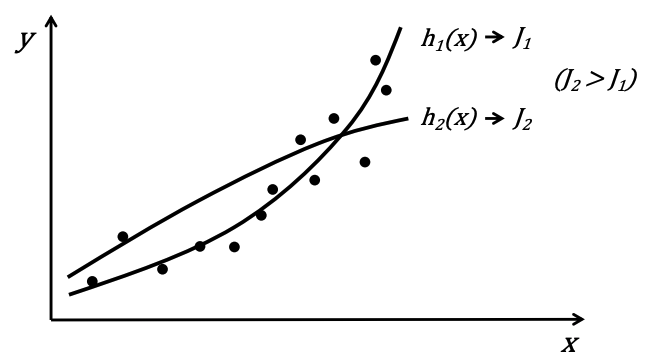
\includegraphics[width=0.8\linewidth]{images/cost-function.png}
    \caption{
        An example of two prediction curves with their associated cost
        functions shown and compared.
    }
    \label{fig:cost-function}
\end{figure}

\begin{definition}[Least squares deviation cost]
    \[
        J(y_i, h(x_i)) = \frac 1n \sum_{i=1}^n (y_i - h(x_i))^2.
    \]
\end{definition}

\begin{definition}[Least absolute deviation cost]
    \[
        J(y_i, h(x_i)) = \frac 1n \sum_{i=1}^n \lvert y_i - h(x_i) \rvert.
    \]
\end{definition}

Least absolute deviation cost is more robust (in regards to outleirs)
but can pose computation challenges when compared to least squares deviation
cost.

\begin{definition}[Huber-M cost]
    \[
        J(y_i, h(x_i)) = \frac 1n \sum_{i = 1}^n
        \begin{cases}
            \frac12 (y_i - h(x_i))^2 & \lvert y_i - h(x_i) \rvert < \delta \\
            \delta (\lvert y_i - h(x_i) \rvert - \frac12 \delta) & \text{otherwise}.
        \end{cases}
    \]
    $\delta$ is a constant that is calculated from some specified 
    percentile of absolute residuals.
\end{definition}

This function is quadratic for small residuals and then linear for larger
values. It is a \emph{hybrid} cost function.

\begin{figure}[]
    \centering
    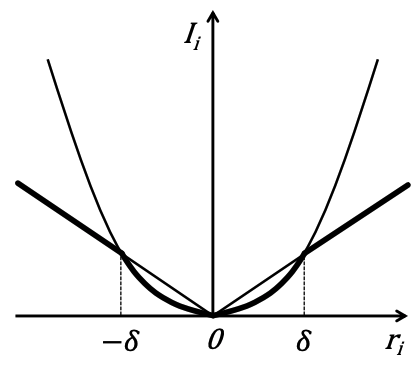
\includegraphics[width=0.8\linewidth]{images/huber-m}
    \caption{
        A graph of the huber loss function.
    }
    \label{fig:huber-m}
\end{figure}

\section{Binary classifiers}

\begin{definition}[Binary classification]
    \textbf{Binary classification} is the task of classifying elements
    of a given set into two groups given a \textbf{classification rule}.
\end{definition}

\section{Performance measures}

In binary classification, how do we \emph{measure} the performance of our model?
We define the true positive $tp$ as the number of correct positive identifications,
false positive $fp$ as the number of incorrect positive identifications,
false negative $fn$ as the number of incorrect negative identifications, and
true negative $tn$ as the number of correct negative identitifications.
We define the \textbf{precision} as
\[
    \operatorname{precision} = \frac{tp}{tp + fp};
\]
the \textbf{recall} (or \textbf{sensitivity}) as
\[
    \operatorname{recall} = \frac{tp}{tp + fn};
\]
and the \textbf{specificity} as
\[
    \operatorname{specificity} = \frac{tn}{tn + fp}. 
\]

\begin{definition}[ROC curve]
    A \textbf{ROC curve} is a measure on the diagnostic ability of a binary
    classification system.
    It is created by plotting
    $\operatorname{sensitivity}$ against
    $1 - \operatorname{specificity}$.
\end{definition}

\begin{figure}[]
    \centering
    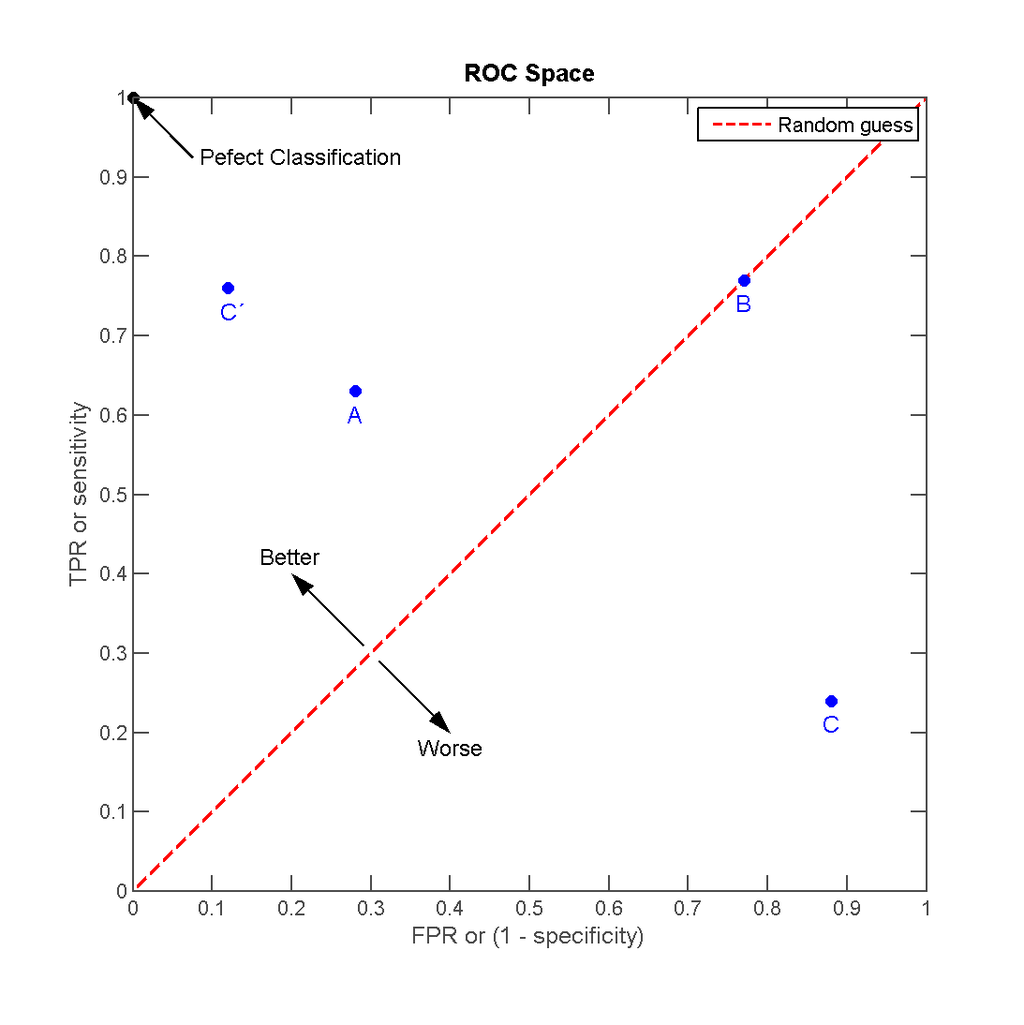
\includegraphics[width=0.8\linewidth]{images/roc-curve.png}
    \caption{A ROC curve.}
    \label{fig:roc-curve}
\end{figure}
